%%%% Report for CSCE 411 Project
\documentclass{article}
\usepackage{amsmath,pgfplots}

%%%% Title Page
\title{CSCE 411 Project Report}
\author{Daniel Bartel}
\date{}



\begin{document}
  \maketitle
  \section*{Problem Description}
  The chosen problem was the single-source shortest path problem. Given a weighted graph, the shortest path algorithm will compute the shortest paths from a given node to every other node in the graph.
\\ \ \\
Shortest path algorithms can have many real world applicatoins including:
\begin{enumerate}
  \item[\textbullet] Driving Directions
  \item[\textbullet] AI Path finding
  \item[\textbullet] Routing data through a network
\end{enumerate}
  \section*{Algorithm Overview}
  The two competing algorithms were Dijkstra's algorithm and the Bellman-Ford algorithm. Both algorithms use the idea of ``relaxing'' edges, which involves calculating approxmiate distances and replacing them with more accurate values until the correct solution is reached.
    \subsection*{Bellman-Ford}
    The Bellman-Ford algorithm was published in 1958 by Richard Bellman and in 1956 by Lester Ford Jr. The algorithm approaches the single source shortest path problem from a dynamic programming perspective. The algorithm executes the following steps: (d[u] is the distance to vertex u, w(u,v) is the weight of the edge (u,v), parent[u] is the parent node of [u] in a shortest path)
    \begin{enumerate}
      \item[1.] \textbf{Initialization}
        \begin{enumerate}
        \item[(a)] For all vertices that aren't the source: set the d[u] to infinity , and the parent[u] to nil
        \item[(b)] Initialize the source d[s] = 0, and the parent[s] to s
        \end{enumerate}
      \item[2.] \textbf{For each vertext v in V: Relax Edges}\\
        Relaxing edges works as follows: for an edge (u,v):\\
         if $d[u] + w(u,v) < d[v]$ then\\
            $d[v] = d[u] + w(u,v)$\\
            parent[v] $= u$
      \item[3.] Return the shortest paths
    \end{enumerate}
    The Bellman-Ford algorithm runs in $O(|V| * |E|)$ time. However, if given a directed acyclic graph, Bellman-Ford can run in $O(|V| + |E|)$ time if the graph is topologically sorted prior to execution of Bellman-Ford.
    \subsection*{Dijkstra}
Dijkstra's algorithm was first published by Edsger Dijkstra in 1959. This algorithm is a greedy algorithm; the closest vertex will always be the vertex that is evaluated next. Dijkstra's algorithm executes in the following manner:
    \begin{enumerate}
      \item[1.] \textbf{Initialization} Initialization is the same as the Bellman-Ford algorithm with one exception: the all vertices are stored in a priority queue Q, where the priority of each vertex is its distance.
      \item[2.] \textbf{While Q is not empty:} Extract the minimum node from Q, relax its edges\\
        Relaxing edges operates in the same manner as the Bellman-Ford with one small addition. If a vertice's distance is changed, it also has its priority in Q decreased as the priorities in the queue are based on distance.
      \item[3.] Return the shortest paths
    \end{enumerate}
The run time of Dijkstra's algorithm depends on the implementation of the priority queue. Using a simple, unsorted array, the run time is $O(V^2)$. If the queue is implemented in a binary heap, the running time will be $O(E \log V)$.  For this project, Dijkstra's algorithm was implemented using an unsorted array.
Dijkstra's algorithm does not work for graphs with negatively weighted edges. This is because of the greedy nature of the algorithm. Once a vertex has been pulled from the priority queue, the algorithm assumes the minimum distance to that vertex has been found. With negatively weighted edges this may not always be the case. On the other hand, Bellman-Ford will work for negatively weighted graphs.
  \section*{Implementation}
The algorithms were implemented in Common Lisp. In addition to the attached source code, the project is available on GitHub: \textit{https://github.com/dbartel/411project}. 
  \section*{Data}
The running time for both of these algorithms depends on two things: the number of vertices and the number of edges in a graph. So, the execution time was measured while varying these two factors.\\
The following data tables show the results of the tests. Timing was performed using the built in Common Lisp macro (time), measured in seconds. For the tests varying the number of edges, each graph had 500 vertices.\\
\begin{center}
\begin{tabular}{|c|c|c|}
\hline
Vertex Total & Bellman-Ford & Dijkstra \\
\hline
100 & 0.01 & 0.004 \\
\hline
200 & 0.071 & 0.045 \\
\hline
400 & 0.548 & 0.399 \\
\hline
800 & 4.315 & 2.121 \\
\hline
1000 & 8.430 & 6.151 \\
\hline
\hline
Edge Total & Bellman-Ford & Dijkstra \\
\hline
100 & 1.075 & 0.738 \\
\hline
200 & 1.077 & 0.442 \\
\hline
400 & 1.077 & 0.615 \\
\hline
800 & 1.078 & 0.463 \\
\hline
1000 & 1.078 & 0.459 \\
\hline
\end{tabular}
\\ \ \\
\textbf{Vertex Test Graph}\\
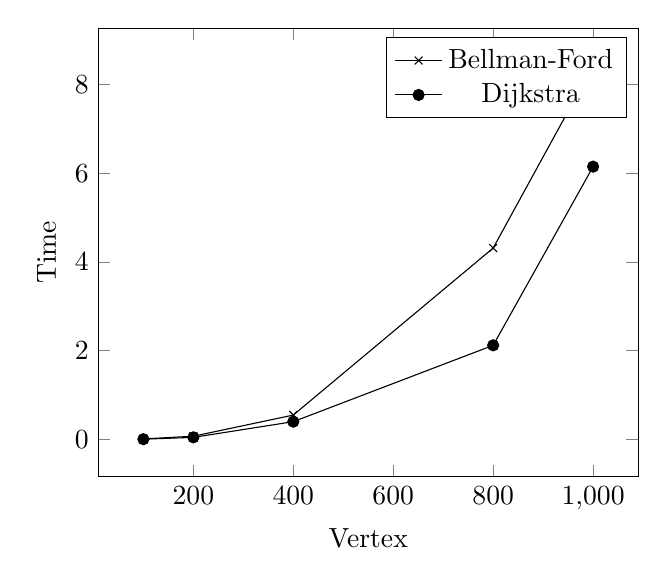
\begin{tikzpicture}
  \begin{axis} [
    xlabel=Vertex,
    ylabel=Time]
    \addplot[color=black,mark=x] coordinates {
      (100,0.01)
      (200,0.071)
      (400,0.548)
      (800,4.315)
      (1000,8.430)
    };

    \addplot[color=black,mark=*] coordinates {
      (100,0.004)
      (200,0.045)
      (400,0.399)
      (800,2.121)
      (1000,6.151)
    };
    \legend{Bellman-Ford,Dijkstra}
  \end{axis}
\end{tikzpicture}
\newpage
\textbf{Edge Test Graph}\\
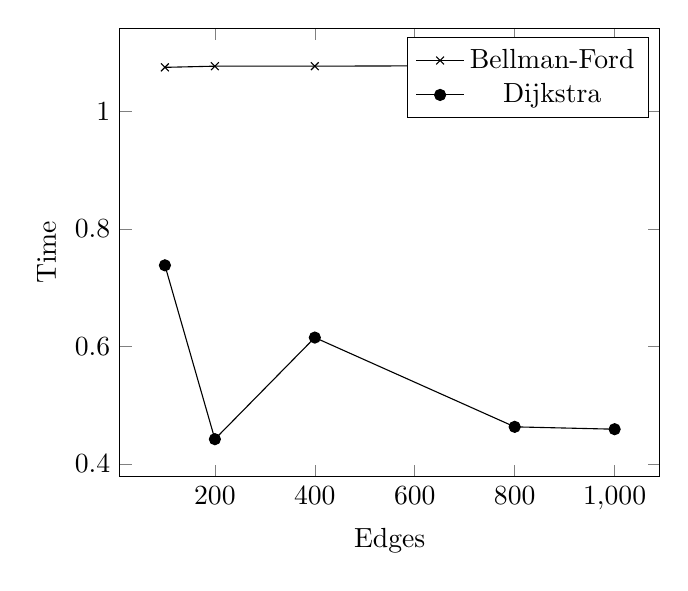
\begin{tikzpicture}
  \begin{axis} [
    xlabel=Edges,
    ylabel=Time]
    \addplot[color=black,mark=x] coordinates {
      (100,1.075)
      (200,1.077)
      (400,1.077)
      (800,1.078)
      (1000,1.078)
    };

    \addplot[color=black,mark=*] coordinates {
      (100,0.738)
      (200,0.442)
      (400,0.615)
      (800,0.463)
      (1000,0.459)
    };
    \legend{Bellman-Ford,Dijkstra}
  \end{axis}
\end{tikzpicture}\\

\end{center}
\section*{Conclusion}
The ``real-world'' results supported the asymptotic analysis. Dijkstra's algorithm performed better than the Bellman-Ford algorithm in both situations. For both algorithms, the asymptotic analysis shows the run time growing with the number of vertices and the number of edges. The tests showed this as well.
\\ \ \\
Both of these algorithms can be improved in a number of ways which were not tested during this project. For example, Bellman-Ford can run in linear time if the graph is a topologically sorted DAG. Also, Dijkstra's run time can be improved if implementing a priority queue as a binary heap instead of an unsorted array. Even with these improvements though,  for positively weighted graphs, Dijkstra's algorithm will run faster than the Bellman-Ford algorithm. Bellman-Ford has the advantage of working with negatively weighted edges.
\\ \ \\
From an implementation perspective, neither algorithm was noticeably more difficult to write than the other. Both utilize the same basic steps, the main difference being the order in which the vertices are processed. So, if choosing between the two algorithms, the decision rests almost entirely on the existence of negatively weighted edges. 

\end{document}
